\documentclass[tikz]{standalone}

% \usepackage{newtxtext,newtxmath}

%!TEX root = main.tex

% mytikzset
\usepackage{tikz}
\usetikzlibrary{positioning,arrows,shapes,patterns}
\usetikzlibrary{decorations.pathmorphing}
\usetikzlibrary{decorations.markings}
\usetikzlibrary{decorations.pathreplacing}
\usetikzlibrary{calc}
\usetikzlibrary{patterns}
\usetikzlibrary{decorations.markings}
\usetikzlibrary{petri}

\tikzset{
  vector/.style={thick,double,draw=black, postaction={decorate},
    decoration={markings,mark=at position .6 with {\arrow[black,scale=0.4]{triangle 45}}}},
  axial/.style={thick,double,densely dashed,draw=black, postaction={decorate},
    decoration={markings,mark=at position .6 with {\arrow[black,scale=0.4]{triangle 45}}}},
  gluon/.style={decorate, draw=black,
    decoration={coil,aspect=0.3,segment length=5pt,amplitude=3pt}},
  pseudo/.style={thick, dashed, draw=black, postaction={decorate},
    decoration={markings,mark=at position .6 with {\arrow[red,scale=0.5]{triangle 45}}}},
  scalar/.style={thick,draw=black, postaction={decorate},
    decoration={markings,mark=at position .6 with {\arrow[black,scale=0.5]{triangle 45}}}},
  cut/.style={draw=black, decorate, decoration={snake, segment length=1mm, amplitude=0.2mm}}
}

\usetikzlibrary{decorations.pathreplacing}

\begin{document}
\nopagecolor
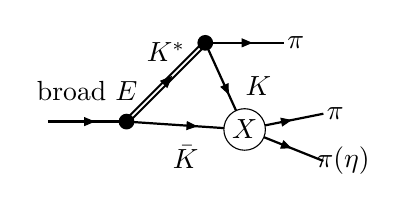
\begin{tikzpicture}[baseline=0.cm]
  \draw[scalar] (0,0) -- node [label=above:{broad $E$}] {} (1,0);
  \draw[vector] (1,0) -- node [label=above:{$K^*$}] {} (2,1);
  \fill[black]  (1,0) circle [radius=0.1];
  \draw[scalar] (1,0) -- node [label=below:{$\bar{K}$}] {} (2.5,-0.1);
  \fill[black]  (2,1) circle [radius=0.1];
  \draw[scalar] (2,1) -- (3,1);
  \draw[scalar] (2,1) -- node [label=right:{$K$}] {} (2.5,-0.1);
  \node[] () at (3.15,1) {$\pi$};
  \draw[scalar] (2.5,-0.1) -- (3.5,0.1);
  \draw[scalar] (2.5,-0.1) -- (3.5,-0.5);
  \node[] () at (3.65,0.1) {$\pi$};
  \node[] () at (3.75,-0.5) {$\pi(\eta)$};
  \node[circle,draw,inner sep=0pt,minimum size=15pt, fill=white] () at (2.5,-0.1) {$X$};
\end{tikzpicture}
\end{document}
